%Wir verwenden eine DIN-A4-Seite und die Schriftgröße 12.
\documentclass[a4paper,12pt]{scrartcl} 


%Diese drei Pakete benötigen wir für die Umlaute, Deutsche Silbentrennung etc.
%Apple-Nutzer sollten anstelle von \usepackage[latin1]{inputenc} das Paket \usepackage[applemac]{inputenc} verwenden
%% \usepackage[latin1]{inputenc}
%%apt-get install texlive-lang-german damit ngerman keine Probleme mehr macht !!
%\usepackage[utf8]{inputenc} 
%\usepackage[T1]{fontenc}
%\usepackage[ngerman]{babel}

%Das Paket erzeugt ein anklickbares Verzeichnis in der PDF-Datei.
%\usepackage{hyperref}

%Das Paket wird für die anderthalb-zeiligen Zeilenabstand benötigt
\usepackage{setspace}

%%HTWM-Vorlage - benoetigt apt-get install texlive-fonts-extra
\setcounter{tocdepth}{3}				%Schatelungstiefe Inhaltsverz.
\usepackage[utf8]{inputenc}			%deutsche Umlaute
\usepackage{german, ngerman}
\usepackage[ngerman]{babel}			%Rechtschreibprüfung
\usepackage{color,listings} 			%Quellcode Highlighting, bindet das
%Paket Listings ein
\usepackage{listings}
\usepackage{color}
\usepackage{textcomp}
\usepackage[T1]{fontenc}				%srccode
\usepackage[scaled]{beramono}		%srccode
\usepackage{longtable}				%mehrseitige tabellen
\usepackage[tableposition=b]{caption}
\usepackage[pdftex, pdftoolbar=false, hyperfootnotes=false, bookmarks,
bookmarksopen, bookmarksnumbered, bookmarksopenlevel=2, pdfpagelabels=true,
pdfstartpage=3, pdfstartview=FitH,]{hyperref} %Verlinkungen
\usepackage{array}					%farbige Tabellen
\usepackage[table]{xcolor} 			%farbige Tabellen
\usepackage{graphicx}				% \includegraphics bnoetigt dies
%%\usepackage{subfigure} 				%% Bilder nebeneinander einfuegen

\usepackage{fancyhdr, graphicx}		%% Logo auf Titelseite
\renewcommand{\headrulewidth}{0pt}
\fancyhead[L]{}
\fancyhead[R]{
  \includegraphics[width=52mm]{./images/htwk.png}
}

%\usepackage{draftwatermark}			% wasserzeichen
	%Quelle: http://choorucode.com/2010/05/05/latex-adding-draft-watermark/?like=1&source=post_flair&_wpnonce=1c9f85538d
%\SetWatermarkText{VORABVERSION}		% wasserzeichen-text
%\SetWatermarkLightness{0.9}			% wasserzeichen-kontrast
%\SetWatermarkScale{2.5}				% wasserzeichen-zeichengroe\ss{}e

\usepackage{float}					% Bilder mittels H-Paramter genau positionieren
\restylefloat{figure}				% Bilder mittels H-Paramter genau positionieren


\definecolor{Navy}{rgb}{0,0,0.5}
\definecolor{Gray}{gray}{0.5}
\definecolor{dunkelgrau}{rgb}{0.8,0.8,0.8}
\definecolor{hellgrau}{rgb}{0.95,0.95,0.95}
\definecolor{hellgrau2}{rgb}{0.93,0.93,0.93}

\hypersetup{
	colorlinks=true, 			% false: boxed links; true: colored links
	linkcolor=Navy,          		% color of internal links
	citecolor=Gray,        			% color of links to bibliography
	filecolor=magenta,      		% color of file links
	urlcolor=blue,           		% color of external links
	linkbordercolor={1 1 1}, 		% set to white
	citebordercolor={1 1 1} 		% set to white
}


%Einrückung eines neuen Absatzes
\setlength{\parindent}{0em}

%Definition der Ränder
\usepackage[paper=a4paper,left=30mm,right=30mm,top=30mm,bottom=30mm]{geometry}

%Abstand der Fussnoten
\deffootnote{1em}{1em}{\textsuperscript{\thefootnotemark\ }}

%Regeln, bis zu welcher Tiefe (section,subsection,subsubsection) Überschriften angezeigt werden sollen (Anzeige der Überschriften im Verzeichnis / Anzeige der Nummerierung)
%\setcounter{tocdepth}{3}
%\setcounter{secnumdepth}{3}

\fancypagestyle{htwkheader}
{
  \fancyhf{}	% clear all header and footer fields
    \fancyhead[RO]{
	\makebox[\textwidth]{	%% schiebe Logo nach aussen auf den Rand
		\rule{0.9				%% nach aussen schieben hoeherer Wert -> Logo weiter nach aussen
		  \textwidth}{0cm} %% nicht nach unten schieben = 0cm
			\includegraphics*[width=52mm]{./images/htwk.png}	%%Logo HTWK
	  }
  }
}

\makeatletter
\def\ScaleIfNeeded{%
\ifdim\Gin@nat@width>\linewidth
\linewidth
\else
\Gin@nat@width
\fi
}
\makeatother


\begin{document}
%Beginn der Titelseite

\begin{titlepage}
%%\thispagestyle{htwkheader}		
%\addtolength{\voffset}{-2cm}		
%\addtolength{\topmargin}{-2cm}
%\addtolength{\bottommargin}{2cm}
%%%%%%%%%%%%%%%%%%%%%%%%%%%%%%%%%%%%%%%%%%%%%%%%%%%%%%%%%%
%%  Oberer Teil: Links Textblock HTWK, Rechts Logo HTWK %%
%%\begin{figure}[htbp]
%%\begin{minipage}[t]{6cm}	%% linker Teil
%%\vspace{0cm}
HTWK Leipzig\\
Fachbereich IMN \\
Sommersemester 2013
%%\end{minipage}
%%\hfill						%% Zwischenraum auffuellen
%%\begin{minipage}[t]{6cm}	%% rechter Teil
%%\vspace{0pt}
%%\makebox[\textwidth]{	%% schiebe Logo nach aussen auf den Rand
%%  \rule{1				%% nach aussen schieben hoeherer Wert -> Logo weiter nach aussen
%%    \textwidth}{0cm} %% nicht nach unten schieben = 0cm
%%      \includegraphics*[width=52mm]{./images/htwk.png}	%%Logo HTWK
%%}

%%  \end{flushright}
%%\caption{Bild1}			%% keine Bildbeschriftung fuer Logo
%%\label{fig:Bild1}			%% nicht ins Abbildungsverzeichnis aufnehmen
%%\end{minipage}
%%\end{figure}

%\vspace{6cm}

%\addtolength{\voffset}{0cm}

\begin{center}
\begin{Large}
\vfill {\textsf{\textbf{
Beleg im Fach\\Informationssysteme\\
}}}
\end{Large}
Konzeption
\end{center}

\begin{small}
\vfill
Kurt Junghanns, B.Sc.\\
Philipp-Rosenthal-Stra\ss{}e 32\\
04103 Leipzig\\
kurt.junghanns@stud.htwk-leipzig.de\\
\\
Marcel Kirbst, B.Sc.\\
Sieglitz 39 \\
06618 Molau \\
marcel.kirbst@stud.htwk-leipzig.de\\
\\
\today
\end{small}

\end{titlepage}
\addtolength{\voffset}{0cm}

%%%%%%%%%%%%%%%%%%%%%%%%%
%%%Ende der Titelseite%%%
%%%%%%%%%%%%%%%%%%%%%%%%%

%Inhaltsverzeichnis (aktualisiert sich erst nach dem zweiten Setzen)
\tableofcontents

%Beginn einer neuen Seite
\clearpage

%Anderthalbzeiliger Zeilenabstand ab hier
\onehalfspacing

%%\pagestyle{plain}
%\pagestyle{headings}	%% lebende Kopfzeile

%%Abbildungsverzeichnis hier erstellen
\clearpage
\listoffigures

\clearpage
\section{Einleitung}
%%\pagestyle{empty}
Ziel dieses Belegs ist ein Data Warehouse zu erstellen und die Phasen des Data Warehousing zu durchlaufen. Als Datenquellen dienen dabei das soziale Netzwerk Facebook, Geodaten von OpenStreetMap sowie Wetterdaten.\\
Ziel ist die Gewinnung neuer Aussagen anhand der Korrelation dieser Daten.

\clearpage
\section{Beschreibung der Datenquellen}

\subsection{Facebook-API}

Facebook bietet für Entwickler APIs zur Abfrage öffentlicher Profildaten an.
Mit einem eindeutigen Schlüssel ist es möglich diese Daten per HTTP abzufragen.\\
Die Daten werden im JSON-Format ausgeliefert.

\begin{center}
\centering
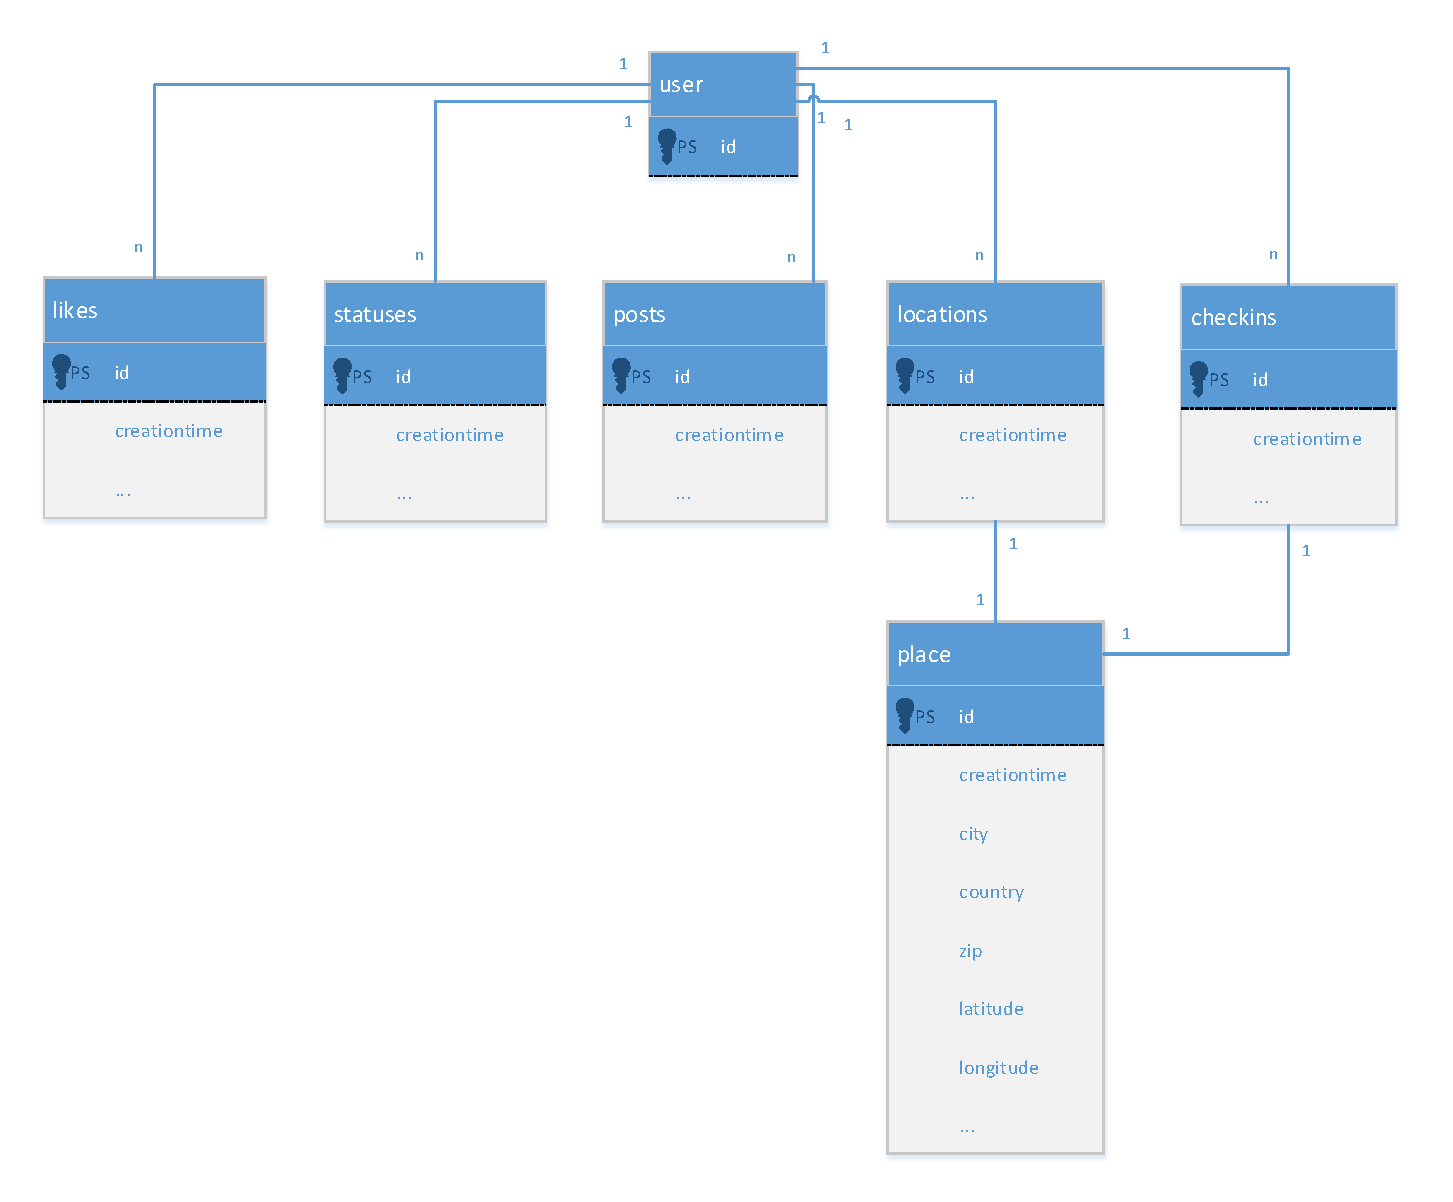
\includegraphics[width=\ScaleIfNeeded]{../user.pdf}%
\captionof{figure}[Facebook Nutzerdaten]{Facebook öffentliche Nutzerdaten}%
\end{center}

Abbildung 1 deutet den Charakter der zu erhaltenten Daten an.\\
Die aufgeführten Attribute und Entitäten sind für die Auswertung essentiell. Die Entitäten und deren Attribute sind jedoch nicht in jedem Datensatz vorhanden.\\
Aus diesem Grund sollen im ETL-Prozess nur Datensätze mit vorhandenen Entitäten und Attributen ausgewertet werden.\\

Zur Abfrage der Nutzer muss eine Zeichenkette zur Filterung mitgegeben werden. Es findet eine Filterung anhand des Nutzernamens statt.\\
In  Folge dessen werden die weltweit häufigsten Namen als weitere Datenquelle herangezogen und damit die Nutzerdaten erhoben.\\

Jede Anfrage liefert einen Ausschnitt der geforderten Daten und Verweise auf die restlichen Daten.


\subsection{OpenStreetMap}

OpenStreetMap bietet neben umfangreichen Kartenmaterial auch den Service, entsprechend eines übergebenen Bereiches die darin befindeten Orte mit diversen Informationen mit HTTP abzurufen.\\
Mit diesem Service sollen fehlende Informationen von Nutzerdaten von Facebook in Bezug auf Positionen und Orte geliefert werden.

\begin{center}
\centering
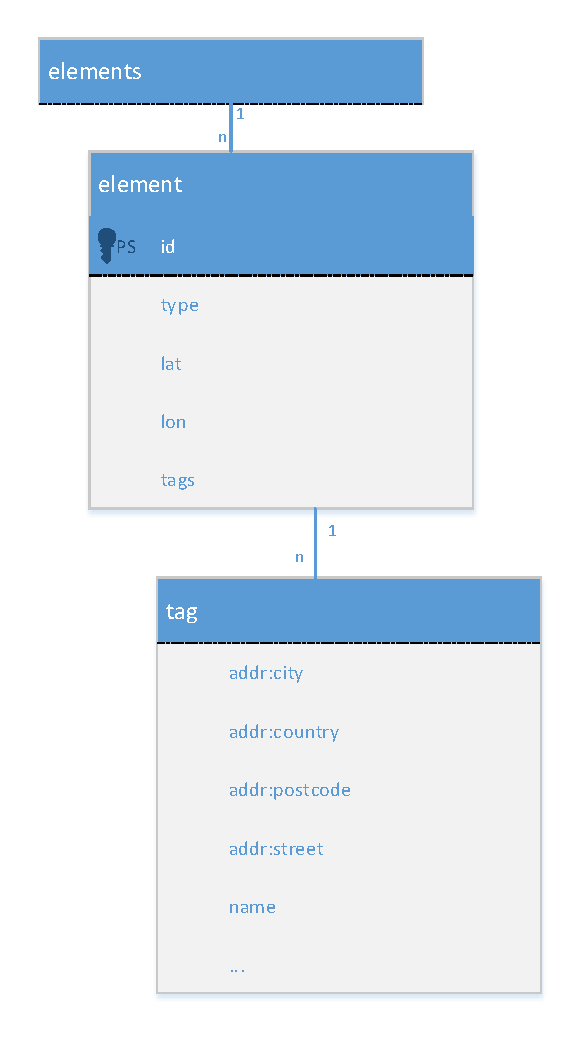
\includegraphics[width=0.5\hsize]{../OSM.pdf}%
\captionof{figure}[OpenStreetMap Orte]{OpenStreetMap Orte}%
\end{center}



\subsection{Wetter-API}

Der Wetterdienst Weather Underground bietet angemeldeten Entwicklern per API Zugriff auf aktuelle und vergangene Wetter- und Klimadaten der ganzen Welt an. Auch hierbei werden die Daten mit HTTP abgefragt und im JSON-Format ausgeliefert.\\
Der Zugriff ist in der kostenlosen Version für Entwickler auf 10 Anfragen pro Minute und 500 Anfragen pro Tag begrenzt.

\begin{center}
\centering
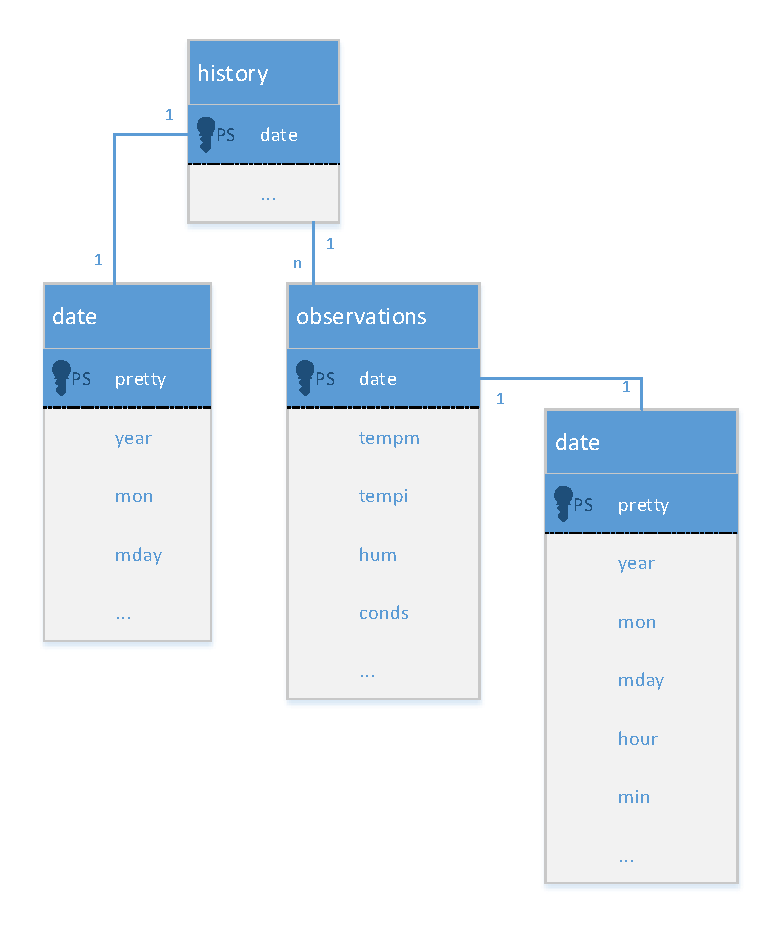
\includegraphics[width=\ScaleIfNeeded]{../Weather.pdf}%
\captionof{figure}[Wetterdaten]{historische Wetterdaten von Weather Underground}%
\end{center}

Das obrige ERM stellt lediglich einen Teil der Granularität und Masse der Daten dar. Die dargestellten Entitäten und Attribute sind für den ETL Prozess relevant.



\subsection{Wetterstationen}

Alle Wetterstationen werden weltweit mit einer global eindeutigen Identifikationsnummer versehen. Eine solche Liste der Wetterstationen, welche auch die Positionskoordinaten enth\"alt, l\"asst sich beispielsweise unter \footnote{\url{http://www.wetterzentrale.de/klima/stnlst.html}} abrufen.

\begin{center}
\centering
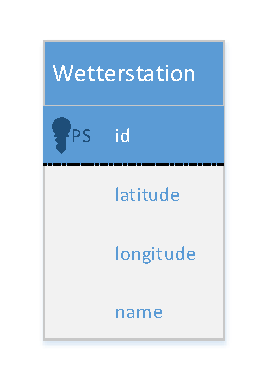
\includegraphics[width=\ScaleIfNeeded]{../Wetterstation.pdf}%
\captionof{figure}[Wetterstationen]{Wetterstationen}%
\end{center}


\section{Architektur des aufzubauenden Data Warehouse}

Die Architektur wurde entsprechend der Vorlesung Informationssysteme entworfen.

\begin{center}
\centering
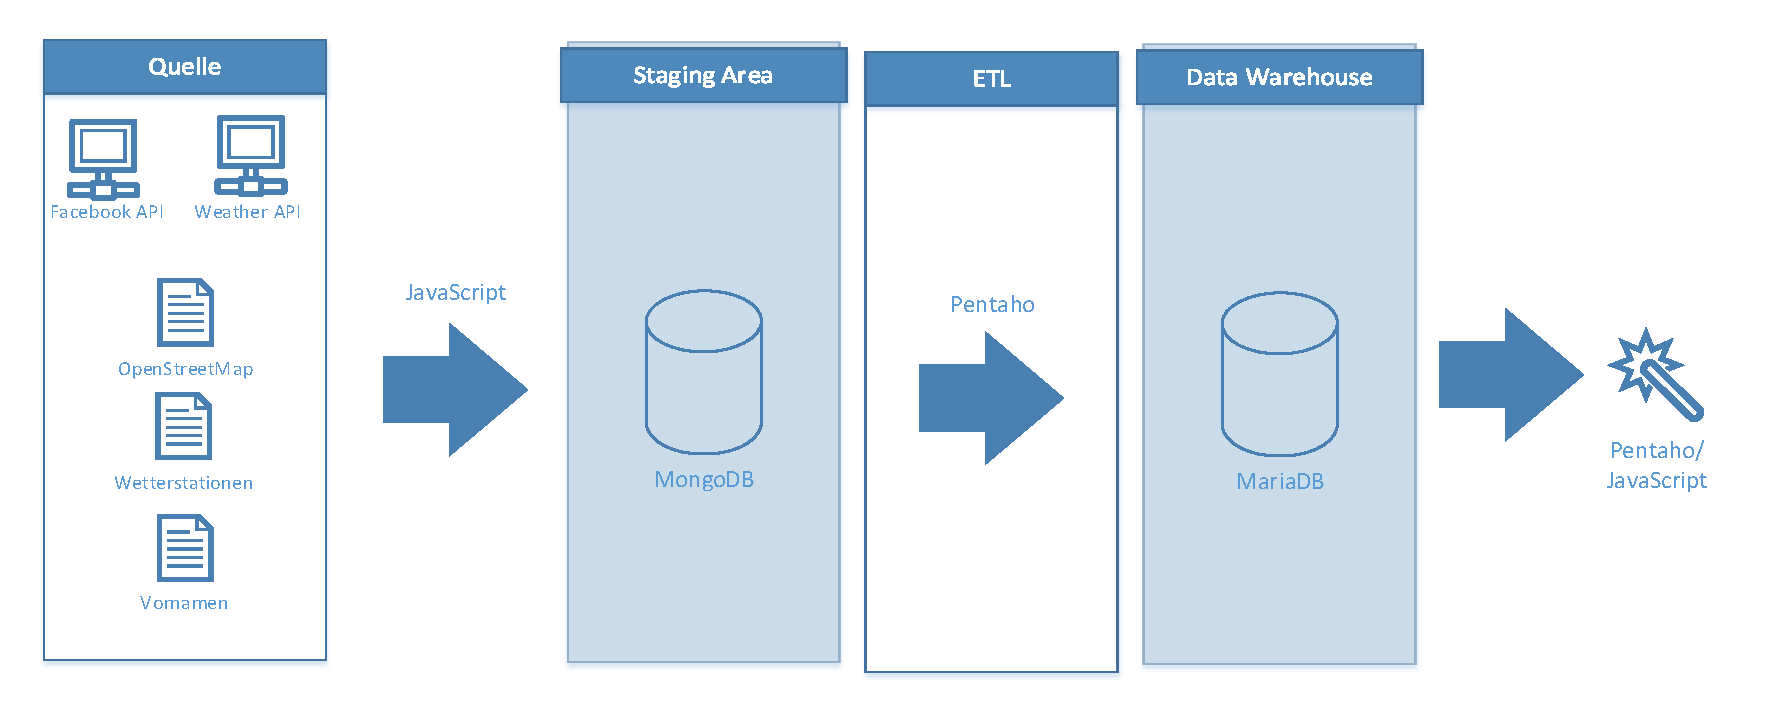
\includegraphics[width=\ScaleIfNeeded]{../Architektur.pdf}%
\captionof{figure}[Architektur Data Warehouse]{Architektur des Data Warehouse}%
\end{center}

Der Zugriff auf große Mengen von Daten mit Hilfe der APIs ist auf Grund des zerstückelten Erhaltes der Daten nur mit einer entsprechenden Logik möglich. Dazu ist es notwendig diese Fragmente zu sammeln.\\
Da die Datenquellen JSON als Format liefern und die Umwandlung in ein solches wenig Aufwand bedarf, wurde als Stating Area die schemafreie dokumentbasierte Datenbank MongoDB verwendet. MongoDB speichert Datensätze im JSON-Format ab. Außerdem wird damit der heterogene Charakter der Quelldaten erhalten und betont.\\

Um den ETL-Prozess übersichtlich zu halten und dessen Definition zu erleichtern, wird das Framework Pentaho verwendet. Pentaho ist eine OpenSource Java Business-Intelligence-Software, welche für die Bereiche ETL, Reporting, OLAP/Analysis und Data-mining geeignet ist.\\

Ein Metadata-Repository ist nicht vorgesehen. Die Definition der Tabellen der MariaDB dienen der Beschreibung der Daten.\\
Eine relationale Abbildung des Data Warehouse wurde gewählt, da die hinter dem Data Warehouse befindliche Geschäftslogik zumeist von relationalen Daten ausgeht.\\

Einfacher halber wird Pentaho zur Auswertung weiter verwendet, wodurch mit geringem Auswand entsprechende Visualisierungen erzeugt werden können. Sollte sich Pentaho nicht eignen, wird zur Auswertung auf JavaScript zurückgegriffen.


\section{Datenbankschemata}



\begin{center}
\centering
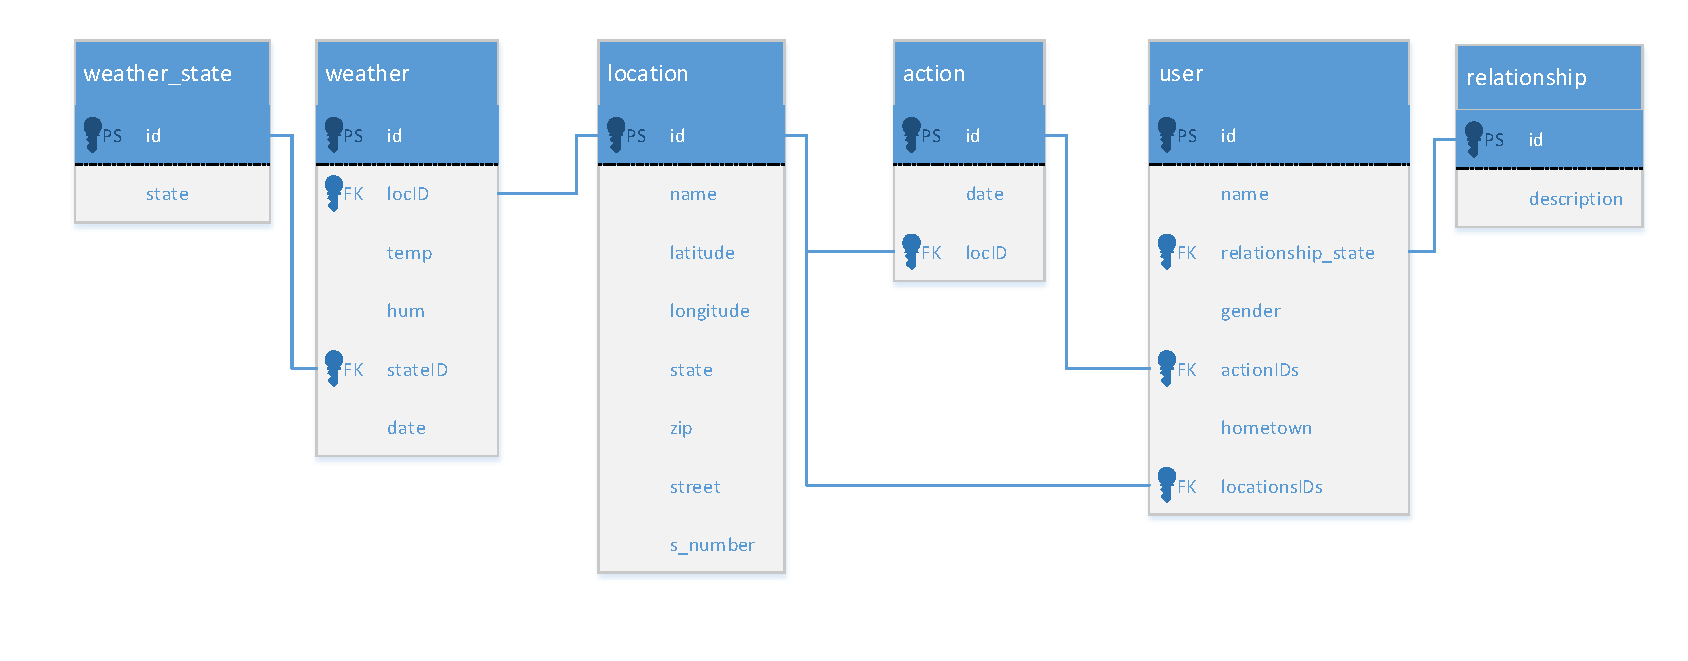
\includegraphics[width=\ScaleIfNeeded]{../Data_Warehouse_ERM.pdf}%
\captionof{figure}[ERM des Data Warehouse]{ERM des Data Warehouse}%
\end{center}




\section{Beschreibung der anvisierten Analysen}

%Die Analysen sollen sich auf der einen Seite auf den Zusammenhang zwischen Beziehungsstatus und Position
Durch Korrelation der vorhandenen Daten soll untersucht werden, ob sich bestimmte Verhaltensmuster abhängig vom Wetter einstellen. Beispielsweise, ob die Aktivitäten der Nutzer mit dem jeweils vorherrschenden Wetter zusammenhängen.\\
Weiterhin ob für geographische Gebiete bestimmte Attribute, wie beispielsweise der Beziehungsstatus, vorherrschen.


%\clearpage
%\section{Glossar}
%\begin{description}
% \item[I2C] Prtokoll zur Kommunikation in Ger\"aten
%\end{description}

\clearpage
\section{Literatur- und Quellenverzeichnis}

\renewcommand\refname{Literaturverzeichnis}
\begin{thebibliography}{999}

\bibitem{buch_datawarehouse}Kiumars Farkisch:  {\sl Data- Warehouse-Systeme kompakt}, Springer Verlag, 2011,
\\ISBN:  978-3-642-21532-2

\end{thebibliography}

\renewcommand\refname{Quellenverzeichnis}
\begin{thebibliography}{999}

%%\cite{citeverweis}
\bibitem{weatherapi}
\url{http://www.wunderground.com/weather/api/d/docs}
\\Abrufbar am 07.05.2013


\bibitem{graphfacebook}
\url{http://developers.facebook.com/docs/reference/api/}
\\Abrufbar am 07.05.2013


\bibitem{pentaho}
\url{http://www.pentaho.de/}
\\Abrufbar am 25.04.2013


\bibitem{OSMAPI}
\url{http://wiki.openstreetmap.org/wiki/Overpass_API/Language_Guide}
\\Abrufbar am 07.05.2013


\bibitem{Wetterstationen}
\url{http://www.wetterzentrale.de/klima/stnlst.html}
\\Abrufbar am 07.05.2013


\end{thebibliography}

\clearpage
%\section{Verzichtserkl\"arung}
%\thispagestyle{plain}

%Hiermit erkläre ich, dass ich die vorliegende Arbeit selbstständig und nur unter Verwendung der angegebenen Literatur und Hilfsmittel angefertigt habe.
%Stellen, die wörtlich oder sinngemäß aus Quellen entnommen wurden, sind als solche
%kenntlich gemacht.\\

%Diese Arbeit wurde in gleicher oder ähnlicher Form noch keiner anderen Prüfungsbehörde vorgelegt.\\\\

%Leipzig, \today
\end{document}
%% EOF